\documentclass[a4,center,fleqn]{NAR}

% Enter dates of publication
\copyrightyear{2008}
\pubdate{31 July 2009}
\pubyear{2009}
\jvolume{37}
\jissue{12}

\bibliography{paper-webserver.bib}

%\articlesubtype{This is the article type (optional)}

\begin{document}

\title{Superphy: Real-time prediction of \textit{E. coli} phenotype using graph-based genome sequence storage and retrieval with the \textit{spfy} module}

\author{%
Corresponding Author\,$^{1,*}$,
First Co-Author\,$^{2}$
and Second Co-Author\,$^2$%
\footnote{To whom correspondence should be addressed.
Tel: +44 000 0000000; Fax: +44 000 0000000; Email: xxx@yyyy.ac.zz}}

\address{%
$^{1}$Affiliation of Corresponding Author
and
$^{2}$Affiliation of Both Co-Authors}
% Affiliation must include:
% Department name, institution name, full road and district address,
% state, Zip or postal code, country

\history{%
Received January 1, 2009;
Revised February 1, 2009;
Accepted March 1, 2009}

\maketitle

\begin{abstract}

\end{abstract}


\section{Introduction}
% new outline
% para
% 1. brief: WGS is standard
% 2. Big Problem: but tools are for individual analysis
% 3. 100,000 genomes, (lookup number for Enterobase, GenBank), how do we run analysis on it
% 4. previous methods (Galaxy/IRIDA: real-time, but no storage of results, other website examples - Denmark?), what problems they addressed
% 5. Problems that remain / lack of result storage means: recomputation, lost data, can't reference old analyses, not suited for "big data"
% 6. Solutions in general: store and increment, huga "big data" analyses, parallelization /queues
% para
% 1. Our specific problem, previous work
% 2. Why solving it is important (for Public health / research)
% 3. how we solved it
% para
% 4. benefits: rapid analyses in real-time -> huge comparisons, replace reference labs -> time & money saved, future work -> expand analyses, more genomes, more species
% 5. analyses modules -> conda -> IRIDA/Galaxy
% 6. short snippit on website link & github link

% 1. brief: WGS is standard
Whole genome sequencing (WGS) can in theory provide the entire genetic content of an organism. This unparalleled resolution and sensitivity has recently transformed public-health surveillance and outbreak response \cite{ronholm2016navigating,lytsy2017time}. Additionally, the identification of novel disease mechanisms \cite{wang2014whole,yuen2015whole}, and rapid clinical diagnoses and reference lab tests based on the specific mechanism of disease are now possible. \cite{willig2015whole,dewey2014clinical}.

% 2. Big Problem: but tools are for individual analysis
The rapid characterization and comparison of bacterial pathogens relies principally on the combination of outputs from multiple software programs that are targeted for specific applications. Examples include the Resistance Gene Identifier (RGI) \cite{mcarthur2013comprehensive} for antimicrobial resistance (AMR) gene prediction, VirulenceFinder \cite{kleinheinz2014applying} for virulence factor (VF) annotation, and Prokka for bacterial genome annotation with external tools \cite{doi:10.1093/bioinformatics/btu153}. In particular, RGI and VirulenceFinder represent a series of \textit{in-silico} methods which have been developed to replicate the results of traditional wet-lab tests; this allows new WGS results to be viewed in the context of historical tests.

Comprehensive platforms that combine individual programs into a cohesive whole also exist. These include free platforms such as the Bacterium Analysis Pipeline (BAP) \cite{thomsen2016bacterial}, the Integrated Rapid Infectious Disease Analysis (IRIDA) project \url{http://www.irida.ca/}, and PATRIC \cite{wattam2013patric}. Commercial applications, such as Bionumerics, which is used by PulseNet international for the analyses of WGS data in outbreak situations also exist, and offer support as well as accredited, standardized tests \cite{swaminathan2001pulsenet}.

% 3. 100,000 genomes, (lookup number for Enterobase, GenBank), how do we run analysis on it
WGS data for bacterial pathogens of public health importance have recently accumulated in public databases in the tens of thousands, with hundreds of thousands set to be available within the next few years. For \textit{Escherichia coli}, there are over sixty thousand publicly available genomes in EnteroBase \url{https://enterobase.warwick.ac.uk/} and three million whole genomes in GenBank \cite{doi:10.1093/nar/gks1195}.

To begin to solve this "big-data" problem, platforms such as BAP and IRIDA provide hosted solutions that compute results in real-time, and distribute analyses across computing resources. While effective for self-contained workflows, many of the comparative analyses that are run are broadly useful, and therefore computed multiple times. An effective method to mitigate the recomputing of analyses is to make the storage and retrieval of results part of the platform, and effectively linked to the organisms of interest with a standardized ontology. Such measures can help ensure the rapid response times required for public health applications, and allow results to be integrated and progressively updated as new data become available.

% 4. Our specific problem, previous work
We have previously developed Superphy \cite{whiteside2016superphy}, an online predictive genomics platform targeting \textit{E. coli}. Superphy integrates pre-computed results with domain-specific knowledge to provide real-time exploration of publicly available genomes. While this tool has been useful for the thousands of pre-computed genomes in its database, the current pace of genome sequencing requires real-time predictive genomic analyses of tens-, and soon hundreds-of-thousands of genomes, and the long term storage and referencing of these results, something that the original SuperPhy platform was incapable of.

% ?. Why solving it is important (for Public health / research)
% Merging points from here into the above sections (2,3,4) to avoid repetition
% - everything is being sequenced (surveillance / outbreak / research)
% - previously mentioned common analyses / want to leverage pre-computed results
% - WGS does not discard old methods, linkage to thousands of historical results by developing in-silico methods of traditional tests
% - need fast / standardized outbreak response
% - need fast / standardized in-silico reference lab
% - need fast / standardized storage and retrieval of results based on ontology
% - all known data can be leveraged, allows the most informed decisions possible
% - etc.

% 5. how we solved it
In this study, we present an update to the SuperPhy platform, called Spfy. Spfy aims to solve the problem of real-time analysis and merging of results from different analysis methods. By merging results and creating links between genome data, Spfy is able to identify relationships between all genomes sequenced in the past, present, and future. This graph-based result storage allows retrospective comparisons as more genomes are sequenced or populations change, and is flexible enough to accomadate new analysis methods as they are developed.

% {needs to be beefed up, in language a biologist / public health worker would care about}

By supporting multiple \textit{in-silico} subtyping options, the platform functions similar to a reference laboratory, with added support for big-data analyses. Subtyping options for E.coli are O-antigen, H-antigen, Shiga-toxin 1 (Stx1), Shiga-toxin 2 (Stx2), and Intimin typing, VF and AMR annotation, pan-genome generation, group comparisons via Fisher's, and machine-learning (ML) based predictions for OmniLog AMR assays. These tasks are divided into subtasks, and distributed across a built-in task queue. Results are also decomposed into graph structures and stored within a larger graph database. By integrating task distribution with graph storage, Spfy enables large-scale analyses, such as epidemiological associations between specific genotypes, biomarkers, host, source, and other metadata, and statistical significance testing of genome markers for user-defined groups. Currently, the platform has been tested with XXX genome files and result storage for XX analyses modules.

Future work will focus on adding additional analyses modules, using machine learning and artificial neural networks to aid genotype to phenotype predictions, and supporting different species. While the integrated approach or storing and retrieving results provides enormous benefits, the developed analyses modules are self-contained and can easily be integrated into existing platforms such as Galaxy \cite{goecks2010galaxy}, and IRIDA. The website is available at \url{https://lfz.corefacility.ca/superphy/spfy/}. Spfy's codebase is provided at \url{https://github.com/superphy/backend} and a developer guide is provided at \url{https://superphy.readthedocs.io/en/latest/}.


% end of new intro

% **************************************************************
% Keep this command to avoid text of first page running into the
% first page footnotes
\enlargethispage{-65.1pt}
% **************************************************************

% Some general comments
% The NAR Database issue is more of a showcase then a rigorous exploration of software design choices.
% Given this focus, i would suggest the following:
% 1. Increase/highlight the discriptions of the functions and capabilities, maybe by adding a Functionality section
% 2. In the Implmentation (or Methods) section, only give a cursory description of the layout and components. Don't need to provide too much justification
% 3. Use the Results section to highlight the scope/size and speed. This can be short
% 4. In the Discussion, this is where i would expand on the justications and reasons for specific design choices. Pick 2-3 main ones and discuss those (i.e. don't need to justify our choice of documentation software). Also compare with other software in Discussion.
% 5. Add a conclusions section


\section{FUNCTIONALITY}
% ONLY FOCUS ON THE ANALYSIS MODULES
% Describe available functions in spfy
% para covering everything
Spfy performs reference laboratory tasks: O-antigen typing, H-antigen typing, and VF gene determination using ECTyper \url{https://github.com/phac-nml/ecoli_serotyping}, STX typing using Phylotyper \cite{whiteside2017phylotyper}, and AMR gene determination using the RGI program \cite{mcarthur2013comprehensive}. Spfy also performs bioinformatics analyses: pangenome generation using Panseq \cite{laing2010pan}, statistical significance testing of genome markers for user-defined groups, and AMR predictions using support vector machines (SVMs).

% para covering ectyper & RGI -- don't really need this
% RGI has its own paper and was in the previous SuperPhy paper
% ectyper will get its own paper
% phylotyper also has its own paper

% group comparisons
Knowledge graphs are a semantic method of linking data points by their relations. Spfy allows users to compare the results associated with particular genome types or metadata by storing all results in a graph structure. Comparisons can be made in real-time, as new genomes are submitted for analysis and the results stored in the existing graph. Any data type in the graph is valid for analysis, such as the presence or absence of pan-genome regions against determined serotypes or other subtyping options. In addition, Spfy supports the submission of user-specified metadata, such as location or source information.

\section{IMPLEMENTATION}
% para: intro to the spfy stack
Spfy's server-side code is developed in Python and the website served to users using the React JavaScript library. For the addition of new data to the database, the following steps are taken:

i) The upload begins through the ReactJS-based website, where user-defined analyses options are selected. The results of these chosen analyses are immediately reported to the user following their completion, while the remaining analyses are subsequently completed and stored in the database without interaction from the user. The public web service accepts up to 200 MB of genome files (50 genomes uncompressed, or 120 genomes compressed).

ii) User-selected analyses are enqueued into the Redis Queue \url{http://python-rq.org/} task queue. Redis Queue consists of a Redis Database \url{https://redis.io/} and task queue workers which run as Python processes.

iii) The workers dequeue the analyses, run them in parallel, and temporarily store results in the Redis database.

iv) Python functions parse the results and permanently store them in Blazegraph \url{https://www.blazegraph.com/}, the graph database used for Superphy.

\subsection{Data Storage}
% para
% 0. Goals: big-data, everything linked, easy addition of new links
% 1. spfy is built around graph technologies
% 1. how we structure our graph
% 2. ontoogies used
% 3. inferencing
% 3 1/2. SPARQL queries
% para: the semantic web
Spfy is built around semantic web technologies which describe the relations between different data \cite{berners2001semantic}. For biological data, individual data points such as genome, contiguous DNA sequence, or gene, are linked together in a query-able graph structure. This allows novel data to be seamlessly incorporated into the existing graph, and has the use of graph databases for relational information has been proposed as a common standard for the open sharing of data \cite{horrocks2005semantic}.

% para: semantic web in spfy
In Spfy, the results from all the analysis modules are converted into graph objects, which are used to update the main graph database. These graph objects, which consist of nodes and edges, must be annotated in order to attribute meaning to these data points. Spfy uses annotations from the GenEpiO \cite{griffiths2017context}, FALDO \cite{bolleman2016faldo}, and TypOn \cite{vaz2014typon} ontologies, as well as custom terminology to enable graph traversals and related data to be inferred from the ontology (see Figure \ref{fig-ontology}). The use of semantic web technologies allows results to be linked to the genomes they were computed from, and for all data points to share a common data structure that can be queried together.

\begin{figure}[t]
\begin{center}
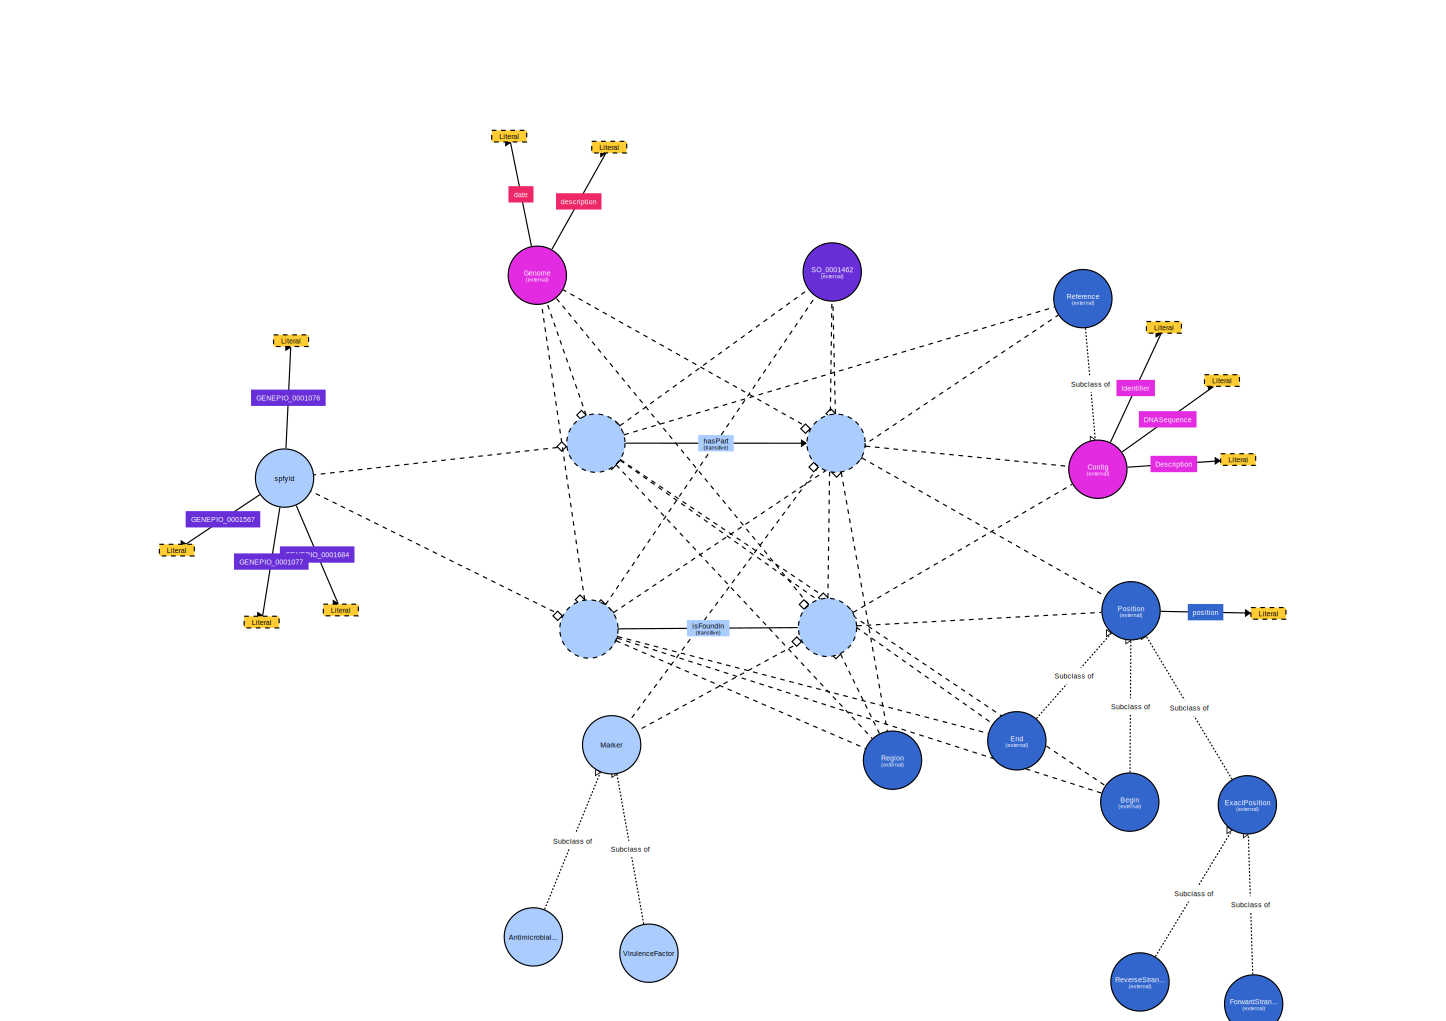
\includegraphics{images/spfy_ontology-1.svg}
\end{center}
\caption{Caption for figure within column.}
\label{fig-ontology}
\end{figure}

% note: below is a feature in development
The permanent storage of results is as a one-time cost, and allows population-wide analyses of all stored genomes; result storage also enables Spfy to avoid recomputation when the same analysis is re-run. To identify analysis tasks, Spfy fingerprints requests by computing its SHA1 hash and tags the results in the graph database with this hash. Subsequent queries are then compared through fingerprinting, and results can be rebuilt from the graph by searching for matching fingerprints.

For population analyses, Spfy searches the graph for all nodes annotated with the queried ontology term. Depending on the given analysis, this data is then typically vectorized into NumPy numerical arrays for use with the SciPy scientific computing library.

\subsection{Web design}
% para
% 1. goals: intuitive/familar, ease of use
% 2. design specs
% 3. Google Material design
% 1. implementation: reactjs, react-md, ES6, JSX
% 4. separation from Flask layer

The front-end website is written using the React JavaScript library \url{https://facebook.github.io/react/} as a single-page application to allow efficient data-flow without reloading the website.
To ensure a familiar user interface, we followed the Material Design specification \url{https://material.io/}, published by Google, surrounding a card-based design.
(see Figure \ref{fig-results})
Both the task selection and results page follow this card-based design: while data storage is actually graph-based, the results of various analysis modules are presented to users in a familiar tabular structure and available for download as .csv files.
(see Figure \ref{fig-tables})

\begin{figure}[t]
\begin{center}
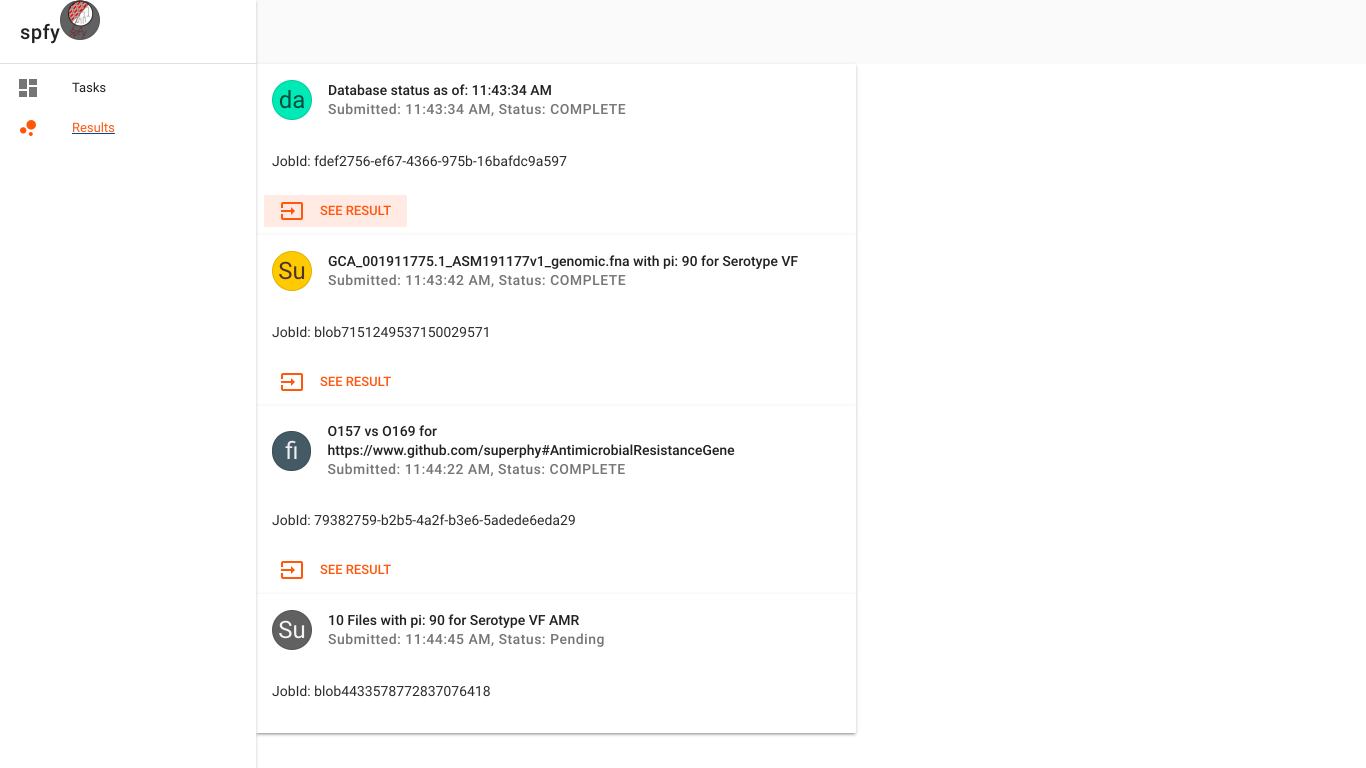
\includegraphics{images/results.png}
\end{center}
\caption{Caption for figure within column.}
\label{fig-results}
\end{figure}

\begin{figure}[t]
\begin{center}
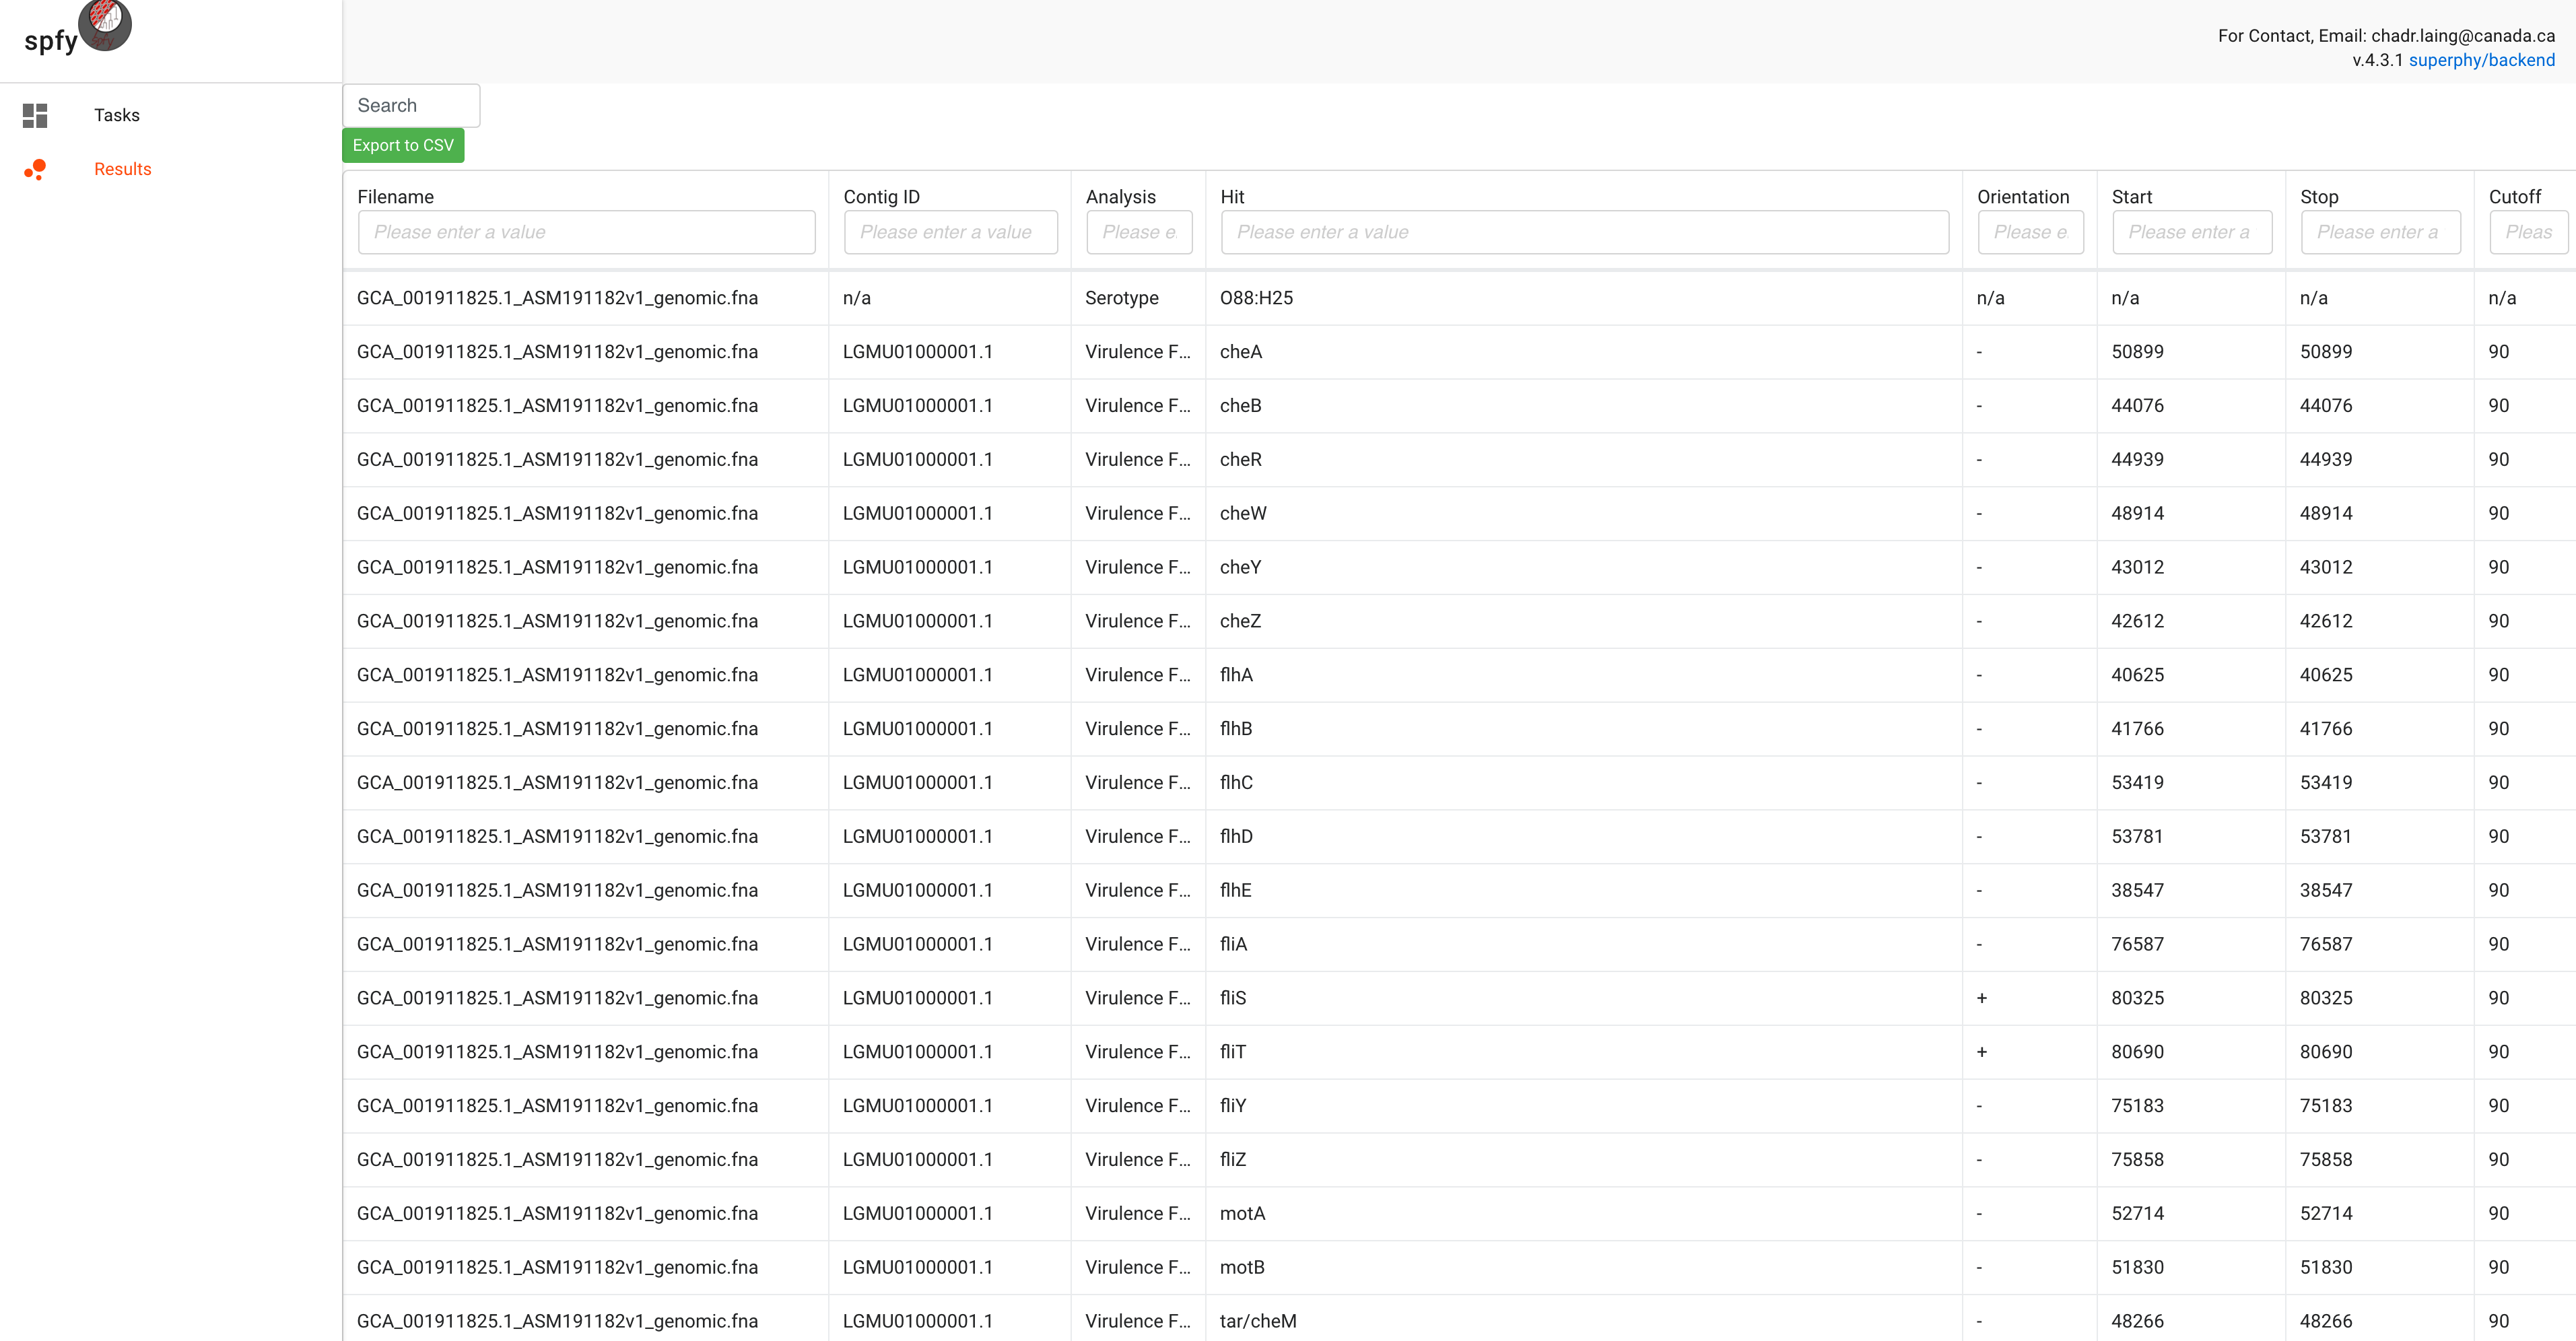
\includegraphics{images/tables.png}
\end{center}
\caption{Caption for figure within column.}
\label{fig-tables}
\end{figure}

\subsection{Real-time analysis pipelines}
% para
% 1. goals: real-time, support for pipelines (linked modules)
% 2. how pipelines have been handled in the past: Galaxy, other examples
% 3. Python, RQ
% para
% 1. how we implemented RQ
%	related: packaging of modules in conda

% para
% 1. goals: scale analyses to "big-data", error handling
% 3. how we handle parallelization with RQ
% para
% 1. how many tasks have we tested this with
% 2. error handling: rq-dashboard, sentry
% 3. why options like sentry are better than traditional logging: scales well to tons (big-data levels) of tasks, groups the same errors together, reporting via email

% para
% 1. goals: why compartmentilizations
% 1. how we implemented docker
% 3. how this lets us replicate worker containers and link everything together

Docker \url{https://www.docker.com/} is a virtualization technology to run self-contained operating systems on the same host computer.
The Spfy platform depends on a series of webservers, databases, and task workers and uses Docker to compartmentalize these services which are then networked together using Docker-Compose \url{https://docs.docker.com/compose/}.
(see Figure \ref{fig-docker})
Docker integration ensures that software dependencies, which typically must be manually installed \cite{doi:10.1093/bioinformatics/btu153,laing2010pan,inouye2014srst2,naccache2014cloud}, are handled automatically, and that service runtimes are compartmentalized; this guarantees that code failures do not propagate to other services.

\begin{figure}[t]
\begin{center}
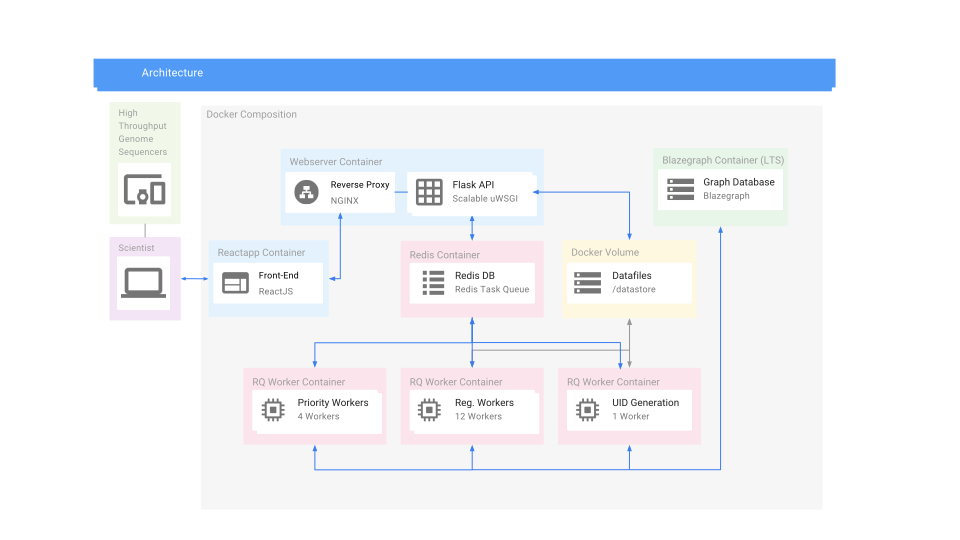
\includegraphics{images/docker.svg}
\end{center}
\caption{Caption for figure within column.}
\label{fig-docker}
\end{figure}

\subsection{Continuous integration and testing}
% Keep this short
% para
% 1. goals: why CI, testing is important
% 2. how we've implemented it, integration with github

TravisCI \url{travisci.io}, a continuous integration (CI) platform, is used to ensure that Spfy \url{https://github.com/superphy/backend} does not break with any changes to the codebase, and runs tests for functionality and backwards compatibility.
The individual tests use PyTest \url{https://doc.pytest.org/}, and are run within TravisCI's virtual environment, and the current build status can be checked either on our Gtihub repository or at \url{https://travis-ci.org/superphy/backend}.
CI is also used to automatically build Spfy's core Docker images, and upload them to Docker Hub \url{https://hub.docker.com/u/superphy/}.

\section{RESULTS}
TODO: Update with all of Enterobase
Spfy was tested with 25,185 public \textit{E. coli} genomes, 5,353 genomes from GenBank and 19,832 genomes from Enterobase, and 55,353 generated samples genomes (267GB), storing both the entire sequences and results for all included analysis modules.
The resulting database had XYZ nodes and XYZ edges, with XYZ object properties, which worked out to XYZ GB of data stored.

% analysis run-time / throughput with different levels of parallelization


\section{DISCUSSION}
% Gist, we address the the "Limitations" of \cite{de2015trends}.
% Namely:
% 1. Custom formats.
% 2. Use of legacy tech (SQL) means youu can't accomadate "Big-Data" goals.

% drawbacks - big data
Many previous bioinformatics software programs have been developed \textit{ad hoc}, with individual researchers and laboratories developing software specific to their environment \cite{de2015trends}.
Such tools were often script-based, with custom data formats, and only suitable for small collections of data \cite{de2015trends}.
While this was acceptable for smaller analyses, bioinformatic pipelines utilizing WGS data are larger and involve linked dependencies, which require the application of systems engineering principles \cite{schatz2015biological}.
Additionally, many subsets of biology now require the analyses of big-data, where the ability to perform computations in real-time, store data in flexible databases, and utilize a common application programming interface (API) linking resources are required \cite{swaminathan2016review}.

One of the key goals in developing Spfy is to maintain instantaneity, as modern websites have accustomed users to immediate results.
We attempt to use innovations in web development to bring a similar experience to Spfy as a predictive genomics platform for \textit{E. coli}.
The use of Docker containerization, task queues, and a graph database, were all chosen to support \textit{instantaneity}; modern analytics platforms must respond to user-requested analyses of big-data in the same efficiency as old analyses of single files.

\subsection{Impact on Public Health Efforts}

% para
% focus on application
The isolation and characterization of bacterial pathogens are critical for Public Health laboratories to rapidly respond to outbreaks, and to effectively monitor known and emerging pathogens through surveillance programs.
Until recently, public-health agencies relied on laboratory tests such as serotyping, pulsed-field gel electrophoresis (PFGE) banding patterns, or Polymerase Chain Reaction (PCR)-based amplification to identify known VFs or AMR genes, along with other tests \cite{ronholm2016navigating}, to characterize bacterial isolates in outbreak and surveillance settings.

AMR testing, VF testing, and Shiga-toxin testing are of particular importance to surveillance efforts as the targets play a key role in a pathogen's lethality to humans.
Current efforts are focused on predictive genomics, where the relevant phenotypic information can be determined through examination of the whole-genome sequence.
WGS methods allow a single laboratory method - the sequencing step - to provide a variety of analysis options, such as AMR, VF, and Shiga-toxin results, and as such can be used to evaluate the spread of outbreaks with better resolution and context than traditional methods \cite{ronholm2016navigating}.

% application: results similar to a wet-lab
Spfy uses WGS results.
After initial sequencing of new isolates, Spfy can be used in place of a traditional reference laboratory, to determine the O-type and H-type, Stx type, and all known VFs and AMR genes in real-time.
These results can be shared with other agencies and researchers over the internet.
Furthermore, using Spfy's database of pre-processed genomes, Spfy can determine all strains a sample may be related to which is useful for monitoring the evolution of pathogens over time.
A computational approach saves the time and cost associated with performing multiple tests per sample, and allows population comparisons which would not be possible with the current pace of WGS results.

\subsection{Comparison with other bioinformatic pipeline technologies}
% trying to cut down on details that would be better suited for the "Implemntation" section.

% namely galaxy
Other scientific workflow technologies such as Galaxy \cite{goecks2010galaxy}, and bioinformatics pipelines IRIDA and BAP are used to run analysis modules on WGS data.
Galaxy aims to provide a reproducible computation-based research environment which is accessible to individuals without programming knowledge. Galaxy tackles the problem of linking different analysis software together, by defining interdependencies using a custom schema. A visual workflow editor is also provided for ease of use.
IRIDA is build on top of the Galaxy framework, and adds prebuilt pipelines specific to bioinformatics uses, as well as sequence and result storage. IRIDA takes a project-based approach, with sequences stored per project, and results store linearly per sequence. Focus is given on refined controls for collaborating on projects, and common terms found in the GenEpiO ontology are used to describe results.

The Bacterial Analysis Platform (BAP), developed out of the Technical University of Denmark provides an integrated analysis pipeline for bacterial WGS data as a web service.
BAP takes a combined approach to genome analysis including different programs, such as for VF and AMR determination, by default into the pipeline.
A record of the different files generated by an analysis are stored in a relational database, and the record is queried to determine which files are returned to the user \cite{thomsen2016bacterial}.

In Spfy, we take a more opinionated approach to result storage and data integration. The benefits of real-time analysis pipelines as found in BAP, and the use of the GenEpiO ontology as in IRIDA, are included in Spfy.
On a per file basis, Spfy performs at a similar speed to BAP on predictive genomics tasks, though Spfy does not provide genome assembly services.
Spfy also processes XXXX files over XX tasks in XXXX time by using a novel approach of distributing computations over a task queue and multiple Docker compartmentalized containers.
In place of a relational database for storing the location of result files, Spfy parses result data into graph objects and integrates results into a persistent graph database.
This enables Spfy to create large datasets where analysis results are linked to genomes, and to perform population-wide analyses. In all, Spfy provides similar functionality with an expanded focus on integrated result storage and big-data analyses.

To approach the challenge of integrating different bioinformatics programs, Spfy instead uses technologies prevalent in common web services not necessarily related to scientific workflows.
While we prefer to package individual bioinformatics programs using language-agnostic package managers such as Conda \url{https://conda.io/}, we do agree that suites of bioinformatics software benefit from having all dependencies installed and deployable in Docker containers \cite{di2015impact}.
These programs are connected to form a workflow using task queues; a design methodology used to offload long-running or non-instantaneous tasks over available computing infrastructure.
Unlike platforms such as Galaxy which favor a drag-and-drop design for building workflows, Spfy favors a tightly coupled approach explicitly linking together different bioinformatics programs within the task queue implementation.
In particular, Spfy uses asynchronous tasks queues which are tripped in response to user requests, thereby allowing immediate responsivity to users on the website, and processes generating human-readable results can be separated from processes handling long-term result storage.

% standard web tech means you can deploy to different cloud computing services
One of the key benefits of using more common-place technologies is the compatibility with other infrastructure resources.
Docker containerization is widely supported by cloud computing services: Amazon Web Services (AWS) \url{https://aws.amazon.com/docker/}, Google Cloud Platform (GCloud) \url{https://cloud.google.com/container-engine/}, and Microsoft Azure \url{https://azure.microsoft.com/en-us/services/container-service/}, and self-hosted cloud computing technologies such as OpenStack \url{https://wiki.openstack.org/wiki/Docker} all support Docker.
% we may want to sign up for a free trial to give an example of this
Spfy packages compute nodes, which manage a collection of task queue workers, as reproducible Docker containers which can be networked together to form a compute cluster.
Docker containerization has a negligible impact on performance \cite{di2015impact}, and allows the platform to easily scale to demand.
In contrast to Galaxy, Spfy is a targeted approach building a predictive analytics platform for \textit{E. coli} which leverages generic web technologies to favor a responsive, big-data design strategy tackling the challenge \cite{fricke2014bacterial} of integrating results from multiple genomes and examining shared connections.
By packaging the individual bioinformatics software as Conda packages, they can be easily ported to Galaxy.

\section{CONCLUSIONS}

\section{ACKNOWLEDGEMENTS}


\subsubsection{Conflict of interest statement.} None declared.
\newpage


\begin{thebibliography}{4}

% Format for article
\bibitem{1}
Author,A.B. and Author,C. (1992)
Article title.
\textit{Abbreviated Journal Name}, \textbf{5}, 300--330.

% Format for book
\bibitem{2}
Author,D., Author,E.F. and Author,G. (1995)
\textit{Book Title}.
Publisher Name, Publisher Address.

% Format for chapter in book
\bibitem{3}
Author,H. and Author,I. (2005)
Chapter title.
In
Editor,A. and Editor,B. (eds),
\textit{Book Title},
Publisher Name, Publisher Address,
pp.\ 60--80.

% Another article
\bibitem{4}
Author,Y. and Author,Z. (2002)
Article title.
\textit{Abbreviated Journal Name}, \textbf{53}, 500--520.

\end{thebibliography}

\end{document}
